\chapter{Aufbau BMD}
\label{cha:Bmd}

BMD Systemhaus GmbH bietet eine ERP(Enterprise Resource Planning)-Gesamtlösung an. Ein Teil davon ist das Modul PPS (Produktionsplanungs- und Steuerungssystem), für das auch die Umsetzung dieser Bachelorarbeit gedacht ist.
Als ERP-Lösungsanbieter ist speziell die Individualisierung für den Kunden von Bedeutung. Oft wird nicht das gesamte System beim Kunden von einen Anbieter realisiert. Aus diesem Grund ist es wichtig, standardisierte Schnittstellen anzubieten, die dennoch leicht an die Anforderungen des jeweiligen Partners angepasst werden können. Im Modul der PPS hat sich BMD dazu entschieden, dies mittels einer XML-Schnittstelle zu realisieren.

\section{PPS-Service}
Der PPS-Service  ist ein Windows-Service der beim Kunden installiert werden kann. Der Service wird über eine .ini-Datei konfiguriert. Auch muss die gewählte Kommunikation in der NTCS definiert werden. Als Möglichkeiten bietet sich ein Dateiaustausch über ein Netzwerklaufwerk und/oder die direkte Kommunikation über TCP/IP. Für TCP/IP gibt es ein definiertes Befehlsprotokoll, das von der externen Seite unterstützt werden muss.
Genutzt wird diese Schnittstelle zum Austausch von Informationen in beiden Seiten. Das bedeutet das damit die Möglichkeit zum Export und Import von Stammdaten als auch Bewegungsdaten besteht. Somit können auch Maschinen und Leitstände angebunden werden. 

\section{Stammdaten}
Beispiele für Stammdaten sind verwaltete Artikel und Stücklisten. Sie repräsentieren echte Artikel die im Betrieb gelagert, verkauft oder produziert werden und deren Zusammensetzung. Die jeweiligen Eigenschaften der Artikel können dann über eine XML-Datei importiert oder exportiert werden vgl. \ref{fig:ArtikelExp}

\begin{figure}
\centering
\lstset{
    language=xml,
    tabsize=3,
    %frame=lines,
    frame=shadowbox,
    rulesepcolor=\color{gray},
    xleftmargin=20pt,
    framexleftmargin=15pt,
    keywordstyle=\color{blue}\bf,
    commentstyle=\color{OliveGreen},
    stringstyle=\color{red},
    numbers=left,
    numberstyle=\tiny,
    numbersep=5pt,
    breaklines=true,
    showstringspaces=false,
    basicstyle=\footnotesize,
    emph={food,name,price},emphstyle={\color{magenta}}}
    \lstinputlisting{images/artikel_export.xml}
\caption{Beispiel für Exportdatei: Artikel.xml  %%\cite{ArtikelExp}.
}
\label{fig:ArtikelExp}
\end{figure}


\section{Bewegungsdaten}
In der Produktion entstehen viele Bewegungsdaten. Dies beginnt bereits bei der Planung der einzelnen Aufträge und endet bei den gelieferten Produkten. Als Beispiel können so von einem automatisierten Produktionsarbeitsplatz gefertigte Produkte an BMD rückgemeldet werden, siehe dazu \ref{fig:ProduktImp}. 

\begin{figure}
\centering
\lstset{
    language=xml,
    tabsize=3,
    %frame=lines,
    frame=shadowbox,
    rulesepcolor=\color{gray},
    xleftmargin=20pt,
    framexleftmargin=15pt,
    keywordstyle=\color{blue}\bf,
    commentstyle=\color{OliveGreen},
    stringstyle=\color{red},
    numbers=left,
    numberstyle=\tiny,
    numbersep=5pt,
    breaklines=true,
    showstringspaces=false,
    basicstyle=\footnotesize,
    emph={food,name,price},emphstyle={\color{magenta}}}
    \lstinputlisting{images/produkt_import.xml}
\caption{Beispiel für Importdatei: Produkt.xml  %\cite{ProduktImp}.
}
\label{fig:ProduktImp}
\end{figure}

\begin{figure}
    \centering
    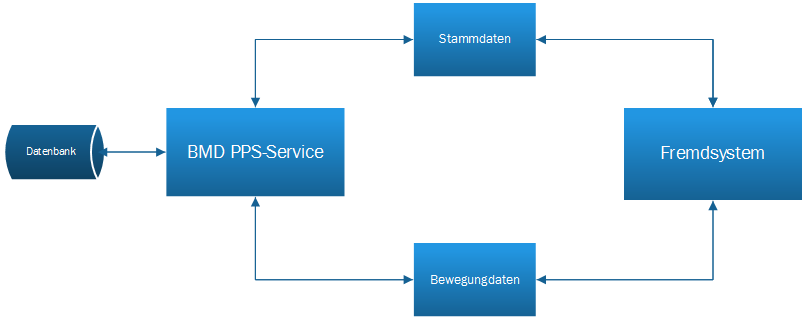
\includegraphics[width=.95\textwidth]{images/Systemschema.png}
    \caption{Arbeitsablauf CAM-Interface}
    \label{fig:Arbeitsablauf}
\end{figure}

\section{Beispiel Kommunikationsablauf}
Ein möglicher Arbeitsablauf beim BMD, wie man in \ref{fig:Arbeitsablauf} kann dann so sein, dass die Stammdaten in BMD gewartet werden. Diese werden anschließend exportiert und vom Fremdsystem eingelesen. Das Fremdsystem erfasst dann die erzeugten Produkte vom Kunden und liefert diese anschließend wieder über eine Exportdatei an BMD. 